\documentclass{article}%
\usepackage[T1]{fontenc}%
\usepackage[utf8]{inputenc}%
\usepackage{lmodern}%
\usepackage{textcomp}%
\usepackage{lastpage}%
\usepackage[head=40pt,margin=0.5in,bottom=0.6in]{geometry}%
\usepackage{graphicx}%
%
\title{\textbf{Guanipa denunció que estuvo detenido este sábado de manera "irregular"}}%
\author{CRISBEL VARELA}%
\date{29/09/2018}%
%
\begin{document}%
\normalsize%
\maketitle%
\textbf{URL: }%
http://www.eluniversal.com/politica/21943/guanipa{-}responsabilizo{-}al{-}gobierno{-}tras{-}ser{-}detenido{-}este{-}sabado\newline%
%
\textbf{Periodico: }%
EU, %
ID: %
21943, %
Seccion: %
politica\newline%
%
\textbf{Palabras Claves: }%
NO\_TIENE\newline%
%
\textbf{Derecho: }%
1.2, %
Otros Derechos: %
1.3, %
Sub Derechos: %
1.2.1, 1.3.2\newline%
%
\textbf{EP: }%
NO\newline%
\newline%
%
\textbf{\textit{El diputado, Juan Pablo Guanipa, explicó que fue interceptado por unas camionetas de la policía por órdenes de Dirwings Arrieta, alcalde de San Francisco y el gobernador del estado Zulia, Omar Prieto}}%
\newline%
\newline%
%
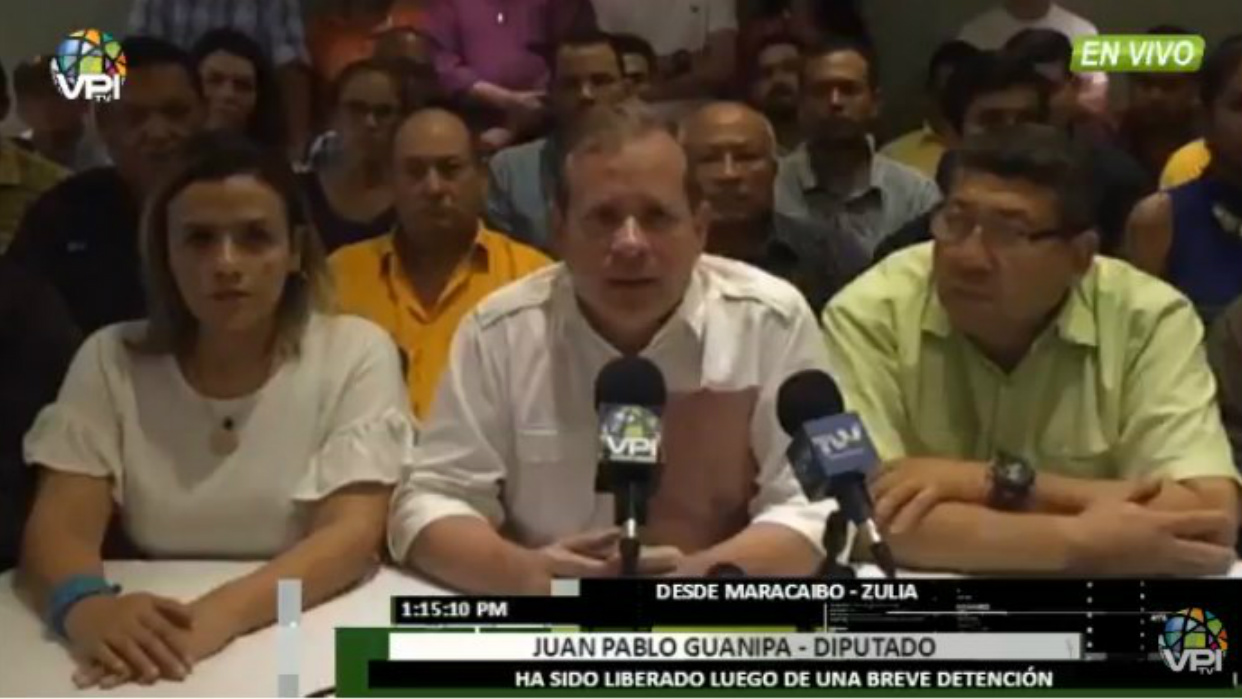
\includegraphics[width=300px]{28.jpg}%
\newline%
%
Caracas.{-}~El diputado a la Asamblea Nacional (AN), Juan Pablo Guanipa, se pronunció tras ser detenido este sábado en horas del mediodía por funcionarios de la policía del municipio San Francisco en el estado Zulia.%
\newline%
%
A través de su cuenta en Twitter, el partido político Primero Justicia (PJ), informó que Guanipa “se encontraba en un acto en el municipio San Francisco mientras grupo irregular irrumpió golpeando a los presentes y llevándose secuestrado al diputado”.%
\newline%
%
Guanipa explicó que fue interceptado por varias camionetas de la policía del sur por órdenes de Dirwings Arrieta, alcalde de San Francisco y el gobernador del estado Zulia, Omar Prieto.%
\newline%
%
Ante los hechos, el parlamentario responsabilizó al presidente de la República, Nicolás Maduro.%
\newline%
%
"Quienes nos interceptaron no tenían uniforme, no tenían identificación, solo tenían armas y con sus armas y sus manos nos golpearon y nos rompieron la ropa" comentó el diputado.%
\newline%
%
Señaló que el alcalde del municipio San Francisco "se disculpó por los excesos de sus funcionarios" a pesar de que estos se comunicaban constantemente con él mientras tenían detenido a Guanipa.%
\newline%
%
Además, Juan Pablo Guanipa agregó que los funcionarios les decían que "si pensábamos que íbamos a hacer actividad política en San Francisco y salir ilesos estábamos equivocados".%
\newline%
%
\end{document}